\documentclass{article}
\usepackage{tabularx}
\usepackage{amsmath}
\usepackage{graphicx}
\usepackage[top = 2cm, bottom = 2cm, right = 2cm, left = 2cm]{geometry}
\usepackage{cite}
\usepackage[final]{hyperref}
\usepackage{listings}
\hypersetup{
	colorlinks=true,
	linkcolor=blue,
	citecolor=blue,
	filecolor=magenta,
	urlcolor=blue         
}

\begin{document}

\title{Practicle 7\\POO with CUDA}
\date{13/02/19}
\maketitle

\begin{abstract}
	
\end{abstract}

\section{Material}
We see on the chapter before that material are basicly just a scatter function. We defined the diffuse material and now we'll focus on metal and dialectric. Create a class material with a virtual pure scatter function. His parameters are the currant ray, the hit structure and the random states. By reference pass the Vector3 attenuation and rayScattered to compute. The return of this function is a boolean.
\begin{lstlisting}
	__device__ virtual bool scatter(
		const Ray& ray,
		const HitInformation& hit,
		Vector3& attenuation,
		Ray& rayScattered,
		curandState* states) const = 0;
\end{lstlisting}

Each sphere in our world will have a material. So we need to add a pointer to material into the sphere class and the HitInformation.
\begin{lstlisting}
	Material* material_;
\end{lstlisting}

And when a ray hit a sphere, we can add the material information into the hit
\begin{lstlisting}
	hit.material_ = material_;
\end{lstlisting}

\subsection{Diffuse material}
Create a class DiffuseMaterial with a inheritance of Material.
\begin{lstlisting}
	class DiffuseMaterial : public Material
\end{lstlisting}

\begin{figure}[h]
	\centering
	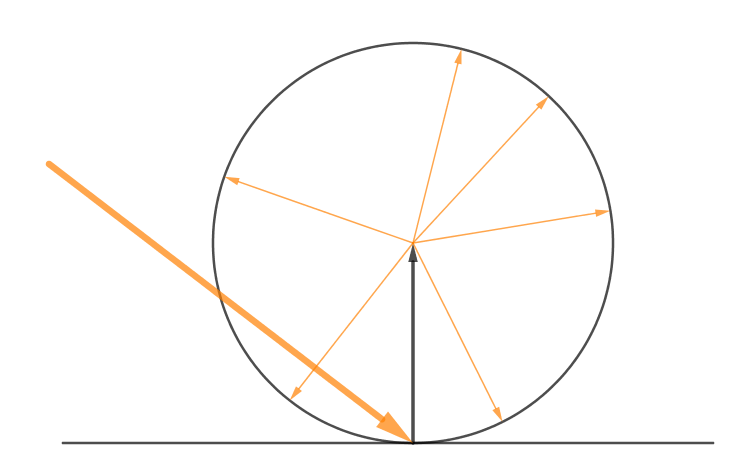
\includegraphics[scale=0.47]{figures/diffuse.png}
	\caption{Absorption}
\end{figure}



\end{document}